\section{Prototyping Semantics}
\label{sec:prototype-semantics:prototyping_semantics}
Figure~\ref{fig:prototype-semantics:languages_overview} shows that connecting \SLCO to existing tools for verification and visualization involves intermediate languages and transformation tools.
Designing this connection and defining its main ingredients required, among others, thorough understanding of the semantics of \SLCO and its specification in terms of basic actions.
Each of these basic actions represents (a part of) an action performed by a particular object or the result of interaction between objects.
The idea behind the intermediate language \CS is to explicitly specify these low-level actions, which are implicit in \SLCO, and to serve as an underlying language to express the semantics of \SLCO.
As a result, \CS together with the transformation~\SLCOtoCS captures the semantics of \SLCO.
All languages and transformations described in this section are available for download\footnote{\url{http://code.google.com/p/prototyping-slco-semantics/}}.

\subsection{Languages}
\label{sec:prototype-semantics:languages}
The process of transforming an \SLCO model into a labeled transition system represented in the language~\LTS is split into three steps.
First, the \SLCO model is simplified, as described in Section~\ref{sec:SLCO:simplified_slco}.
Then, this simplified \SLCO model is translated into a list of configurations and steps, represented in the \CS language.
In this language, we describe the behavior of the entire system, resulting from the communication of the constituting objects, whose behavior is modeled as a set of separate state machines in \SLCO.
Then, this \CS representation is transformed into a list of states and transitions, which form the \LTS representation of the input model.

\subsubsection{CS}
\label{subsucsec:prototype-semantics:cs}
The main ingredients in a \CS description are configurations and steps.
A configuration is a representation of a possible state of the system described by the \SLCO model.
A configuration can make a step, after which the system reaches another configuration.
A step in \CS does not necessarily correspond to a single transition in \SLCO.
Two transitions belonging to two separate objects may lead to a single step in \CS if the statements of these transitions send and receive signals over a synchronous channel and thus allow the two objects to communicate synchronously.
Conversely, a single transition in \SLCO does not necessarily correspond to a single step in \CS.
For an \SLCO transition with a delay statement, several steps (not necessarily executed in sequence) accomplish the behavior specified by the transition.

\begin{listing}
  \lstset{
    language=cs,
    caption=The initial configuration of the running example,
    label=lst:prototype-semantics:configuration,
    numbers=none
  }
  \begin{lstlisting}
    <
     <p, Rec1, Rec1> <p, Rec2, Rec2a> <p, SendRec, SendRec0> <0, q, Com, Com0>,
     [<<q, Com, s>, ""> <<p, SendRec, s>, ""> <<p, Rec1, v>, false> <<p, m>, 0>],
     [<<c2, q, Out2, p, In2>, > <<c1, q, Out1, p, In1>, >],
     initial
    >
  \end{lstlisting}
\end{listing}

\paragraph{Configurations}
Each configuration consists of three mandatory parts and an optional status.
The configuration given in Listing~\ref{lst:prototype-semantics:configuration} is the initial configuration of the model consisting of objects~\SLCOObject{p} and~\SLCOObject{q} shown in Figures~\ref{fig:slco:SLCOExampleCommunication}, \ref{fig:slco:SLCOExampleStructure}, and~\ref{fig:slco:SLCOExampleSMSMinimized}.
The first part of a configuration specifies the current states of all state machines of all objects in the \SLCO model.
This part of the configuration is referred to as the active states of a configuration.
If a state machine~\SLCOStateMachine{sm} of an object~\SLCOObject{o} is currently in state~\SLCOState{st}, this is specified as~\ActiveState{o}{sm}{st} in the active states part of the configuration.
This type of active state is referred to as a plain active state.
Additionally, a second type of active state exists, which is related to delay statements.
These active states are referred to as time-stamped active states.
The time-stamped active state \ActiveStateTimeStamp{5}{o}{sm}{st} denotes that 5~ms have passed since state machine~\SLCOStateMachine{sm} of object~\SLCOObject{o} reached state~\SLCOState{st}.
Furthermore, \ActiveStateTimeStamp{\TSPassed}{o}{sm}{st} denotes that the maximal amount of time specified by the delay statement of any outgoing transition of state~\SLCOState{st} has passed.
The active states part of a configuration consists of a number of plain and time-stamped active states, one for each state machine in the model.

The second part of the configuration, the valuation part, maps variables to values.
In the example configuration in Listing~\ref{lst:prototype-semantics:configuration}, \ValLocal{q}{Com}{s}{``"} expresses that the value of local variable~\SLCOVariable{s} of state machine~\SLCOStateMachine{Com} of object~\SLCOObject{q} is equal to the empty string.
The fact that the value of global variable~\SLCOVariable{m} of object~\SLCOObject{p} is equal to 0 is expressed as \ValGlobal{p}{m}{0}.

The third part of the configuration represents a set of buffers.
For each asynchronous channel in the model, one or two buffers are introduced.
In case of a bidirectional channel, two buffers are introduced, and in case of a unidirectional channel, one buffer is introduced.
The configuration in Listing~\ref{lst:prototype-semantics:configuration} contains two buffers, one for each (unidirectional) channel, and they are both empty.
The first buffer corresponds to channel~\SLCOChannel{c2} and the second buffer to channel~\SLCOChannel{c1}.
Channel~\SLCOChannel{c3} is synchronous and has no corresponding buffer.

The optional status of this configuration is set to \CSStatus{initial} because all state machine are in their initial state.
If all state machines in a configuration are in their final state, the status of this configuration is set to \CSStatus{final}.
Finally, the status of all remaining configurations for which there are no steps to other configurations is set to \CSStatus{deadlock}.

\paragraph{Steps}
The dynamics of the system modeled by a set of communicating objects is represented by steps.
Each step has a source and a target configuration, and an optional label.
A step represents a (basic) action performed by a state machine, the passing of a certain amount of time, or the result of synchronous communication between two objects.
Listing~\ref{lst:prototype-semantics:steps} shows two steps that are part of the \CS representation of the \SLCO model in Figures~\ref{fig:slco:SLCOExampleCommunication}, \ref{fig:slco:SLCOExampleStructure}, and~\ref{fig:slco:SLCOExampleSMSMinimized}.
The first step has a label that represents the reception of the asynchronous signal~\SLCOSignalName{Q} by state machine~\SLCOStateMachine{Rec2}.
The second step represents the transition from state~\SLCOState{SendRec0} to~\SLCOState{SendRec1} of state machine~\SLCOStateMachine{SendRec}, which is enabled because the expression~$\SLCOVariable{m}==6$ holds in the source configuration.
Steps that correspond to the evaluation of an expression, such as this one, have no label.

\begin{listing}
  \lstset{
    language=cs,
    caption=Steps depicting the reception of a signal and the evaluation of an expression,
    label=lst:prototype-semantics:steps,
    numbers=none
  }
  \begin{lstlisting}
    <
     <
      <p, Rec1, Rec1> <p, Rec2, Rec2a> <p, SendRec, SendRec0> <q, Com, Com3>,
      [<<q, Com, s>, ""> <<p, SendRec, s>, ""> <<p, Rec1, v>, false> <<p, m>, 0>],
      [<<c2, q, Out2, p, In2>, <Q, 5>> <<c1, q, Out1, p, In1>, <P, true>>]
     >,
     "receive Q(5)",
     <
      <p, Rec1, Rec1> <p, Rec2, Rec2b> <p, SendRec, SendRec0> <q, Com, Com3>,
      [<<q, Com, s>, ""> <<p, SendRec, s>, ""> <<p, Rec1, v>, false> <<p, m>, 5>],
      [<<c2, q, Out2, p, In2>, > <<c1, q, Out1, p, In1>, <P, true>>]
     >
    >
    <
     <
      <p, Rec1, Rec1> <p, Rec2, Rec2b> <p, SendRec, SendRec0> <q, Com, Com3>,
      [<<q, Com, s>, ""> <<p, SendRec, s>, ""> <<p, Rec1, v>, false> <<p, m>, 6>],
      [<<c2, q, Out2, p, In2>, > <<c1, q, Out1, p, In1>, <P, true>>]
     >,
     <
      <p, Rec1, Rec1> <p, Rec2, Rec2b> <p, SendRec, SendRec1> <q, Com, Com3>,
      [<<q, Com, s>, ""> <<p, SendRec, s>, ""> <<p, Rec1, v>, false> <<p, m>, 6>],
      [<<c2, q, Out2, p, In2>, > <<c1, q, Out1, p, In1>, <P, true>>]
     >
    >
  \end{lstlisting}
\end{listing}

\subsubsection{LTS}
\label{subsubsec:prototyping-semantics:lts}
The language \LTS is a simple language for representing labeled transition systems as a list of states and a list of transitions.
A state can be marked to indicate that it is an initial state, a final state, or a deadlock.
Each transition is described as a pair of states, the source and the target state, and an optional label.
Listing~\ref{lst:prototype-semantics:lts} shows the \LTS description of a tiny labeled transition system  with four states and three transitions.
State~0 is declared as an initial state, state~1 is a deadlock, and state~3 is a final state.
There are three transitions, one of which has label $a$.
The most notable feature of \LTS in comparison to existing languages for the description of labeled transition systems is that \LTS distinguishes between successful termination and deadlock.
Reaching a final state and thus terminating successfully is considered desirable behavior, but reaching a deadlock is not.

\begin{listing}
  \lstset{
    language=lts,
    caption=A small labeled transition system represented in the language~\LTS,
    label=lst:prototype-semantics:lts,
    numbers=none
  }
  \begin{lstlisting}
    states
      initial 0
      deadlock 1
      2
      final 3
    transitions
      0 1
      0 "a" 2
      2 3
  \end{lstlisting}
\end{listing}

\subsection{Tools for Transformation}
Now that the languages used to prototype \SLCO are in place, we describe two of the tools that perform transformations related to these languages.
The first tool produces \CS representations from simplified \SLCO models, and the second tool produces labeled transition systems represented in \LTS from \CS representations.
The tools that perform the transformation from \LTS to \DOT and the transformation from \CS to \DOT are discussed in Section~\ref{sec:prototype-semantics:visualization}, and the simplification of \SLCO is discussed in Section~\ref{sec:SLCO:simplified_slco}.

The aforementioned tools are implemented in the \ASFSDFME~\cite{Brand:2001:ASF}, which is described in Appendix~\ref{ap:tools}.
The main benefits of using the \ASFSDFME for this task are that it offers an IDE for the convenient development of transformations as well as automatic generation of command-line tools.
These command-line tools are fast and make efficient use of memory, which is important when generating \CS and \LTS representations of large state spaces.

\subsubsection{SLCO2CS}

An \SLCO model is translated into \CS in three phases.
First, the initial configuration of the model is constructed.
The list of active states of this configuration consists of the initial states of each of the state machines of the objects in the model, the valuation maps all variables to their initial values, and the buffers corresponding to all asynchronous channels are empty.
Second, the set of all reachable configurations is generated.
This phase is described in more detail below.
Third, the list of configurations is traversed to find the configurations containing only active states that are final and those that have no outgoing steps.
The configurations containing only final active states are marked as final, and the configurations that have no outgoing steps are marked as deadlocks, unless they are already marked as final.

In the second phase, first all configurations that are reachable from the initial configuration are created, as well as all the steps to these configurations.
Then, all configurations that are reachable from these new configurations and the corresponding steps are created, and so on, until no new configuration is found.
The configurations that are reachable from a source configuration are computed based on the active states of this source configuration.
The \ASFSDF functions discussed next are selected from the set of all functions that together implement the generation of configurations and steps within the second phase of the transformation.

Listing~\ref{lst:prototype-semantics:asf_takesteps} shows one of the conditional rewrite rules that implement the function~\ASFFunction{takeStepsFromConfiguration}.
In this rule and all other ASF rules shown in this chapter, variable names start with a dollar sign.
Furthermore, variable names that contain a multiplication symbol~(\texttt{\$X*}) represent lists of terms of a sort,
variable names that contain a plus symbol~(\texttt{\$X+}) represent non-empty lists of terms of a sort,
and variable names that end with a question mark~(\texttt{\$X?}) represent an optional term that can be omitted.
The rule in Listing~\ref{lst:prototype-semantics:asf_takesteps} shows that the computation of possible steps from a given configuration is split into two parts.
First, function~\ASFFunction{takeTimeStepsFromConfiguration} computes a step that represents the passing of a certain amount of time, if such a step is possible from the given configuration.
This computation deals with transitions with delay statements only.
Then, function~\ASFFunction{takeStepsActiveStates} inspects all outgoing transitions of the active states of the source configuration to compute the rest of the reachable~configurations.

\begin{listing}
  \lstset{
    language=asf,
    style=asf,
    caption=ASF rule that computes reachable configuration and the corresponding steps,
    label=lst:prototype-semantics:asf_takesteps,
    numbers=none
  }
  \begin{lstlisting}
    <$Configuration*0, $Step*0> :=
      takeTimeStepsFromConfiguration($Model, $Configuration),
    $ActiveState* := activeStates($Configuration),
    <$Configuration*1, $Step*1> :=
      takeStepsActiveStates($Model, $Configuration, $ActiveState*)
    ====>
    takeStepsFromConfiguration($Model, $Configuration) =
    <$Configuration*0 $Configuration*1, $Step*0 $Step*1>
  \end{lstlisting}
\end{listing}

The ASF rule in Listing~\ref{lst:prototype-semantics:asf_time} shows how a step representing the passing of time is computed.
The function~\ASFFunction{getSmallestTimeStepFromConfiguration} inspects all outgoing transitions of the active states of the given configuration and returns a natural number.
This number is computed from the time stamps of time-stamped active states and the outgoing transitions of these active states.
By construction, all active states that have an outgoing transition with a delay statement also have a time stamp.
For each of the time-stamped active states, function~\ASFFunction{getSmallestTimeStepFromConfiguration} uses their time stamp to compute the smallest amount of time that must pass for one of the delay statements of the related outgoing transitions to become unblocked.
After this amount of time is computed, the resulting configuration and step are constructed by updating the time stamps of all time-stamped active states.

\begin{listing}
  \lstset{
    language=asf,
    style=asf,
    caption=ASF rule that computes a step representing the passing of time,
    label=lst:prototype-semantics:asf_time,
    numbers=none
  }
  \begin{lstlisting}
    canTakeTimeStepFromConfiguration($Model, $Configuration) == true,
    $NatCon := getSmallestTimeStepFromConfiguration($Model, $Configuration),
    $Configuration0 := updateTimeStamps($Model, $Configuration, $NatCon),
    $StrCon := natCon2StrCon($NatCon) || " ms",
    $Step := <$Configuration, $StrCon, $Configuration0>
    ====>
    takeTimeStepsFromConfiguration($Model, $Configuration) =
    <$Configuration0, $Step>
  \end{lstlisting}
\end{listing}

Figure~\ref{fig:prototype-semantics:delays} and Listing~\ref{lst:prototype-semantics:time_steps} illustrate the computation performed by the ASF rule in Listing~\ref{lst:prototype-semantics:asf_time}.
In the initial configuration, the leftmost state machine in Figure~\ref{fig:prototype-semantics:delays} is in state~\SLCOState{A0}, and the rightmost state machine is in state~\SLCOState{B0}.
Both states have a time stamp equal to 0.
The smallest amount of time that must pass for one of the delay statements to become unblocked is 1~ms.
The first step in Listing~\ref{lst:prototype-semantics:time_steps} corresponds to the passing of this amount of time.
In the resulting configuration, the smallest amount of time that must pass for one of the remaining delay statements to become unblocked is 2~ms, which is represented by the second step in Listing~\ref{lst:prototype-semantics:time_steps}.
In the resulting configuration, both delay statements of the leftmost state machine are unblocked, which is indicated by the keyword~\TSPassed in the time-stamped active state~\ActiveStateTimeStamp{\TSPassed}{a}{A}{A0}.
Finally, for the remaining delay statement to become unblocked, 3~ms must pass, as shown in the third step in Listing~\ref{lst:prototype-semantics:time_steps}.

\begin{figure}[hbt]
\centering
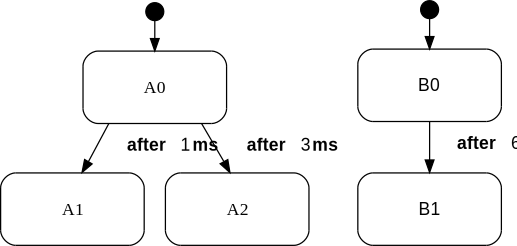
\includegraphics[scale=.45]{prototype-semantics/figs/delays}
\caption{Two state machines with delay statements}
\label{fig:prototype-semantics:delays}
\end{figure}

\begin{listing}
  \lstset{
    language=cs,
    caption=Steps representing the passing of time,
    label=lst:prototype-semantics:time_steps,
    numbers=none
  }
  \begin{lstlisting}
    <
     <<0, a, A, A0> <0, b, B, B0>, [], []>,
     "1 ms",
     <<1, a, A, A0> <1, b, B, B0>, [], []>
    >
    <
     <<1, a, A, A0> <1, b, B, B0>, [], []>,
     "2 ms",
     <<passed, a, A, A0> <3, b, B, B0>, [], []>
    >
    <
     <<passed, a, A, A0> <3, b, B, B0>, [], []>,
     "3 ms",
     <<passed, a, A, A0> <passed, b, B, B0>, [], []>
    >
  \end{lstlisting}
\end{listing}

After constructing the reachable configurations and the corresponding steps related to time, all other configurations that are reachable from the source configuration are computed by the function \ASFFunction{takeStepsActiveStates}, as mentioned above.
For each active state in a configuration, the outgoing transitions are inspected.
Whether a transition is enabled depends on the valuation of the variables, the contents of the buffers, and the values of the optional time stamps.
The valuation of the variables is used to determine whether the expressions of transitions hold, the content of the buffers to determine whether any signal receptions are possible, and the time stamps to determine which delay statements are no longer blocked.

\begin{listing}
  \lstset{
    language=asf,
    style=asf,
    caption=Computing the configuration that is reached after executing an assignment,
    label=lst:prototype-semantics:assign,
    numbers=none
  }
  \begin{lstlisting}
    $ActiveState0 := getNextState($Model, $ActiveState, $Transition),
    $IdCon0 := getObjectId($ActiveState),
    $IdCon1 := getStateMachineId($ActiveState),
    $AssignmentStatement := getStatement($Transition),
    <$Configuration0, $Step0> := processAssignmentStatement(
      $AssignmentStatement, $ActiveState, $ActiveState0, $Configuration,
      $IdCon0, $IdCon1
    )
    ====>
    takeStepTransition($Model, $Configuration, $ActiveState, $Transition) =
    <$Configuration0, $Step0>
  \end{lstlisting}
\end{listing}

Listing~\ref{lst:prototype-semantics:assign} shows one of the conditional rewrite rules that implements the function~\ASFFunction{takeStepTransition}.
This function is used by the function~\ASFFunction{takeStepsActiveStates} to construct the reachable configurations and the corresponding steps for each of the enabled outgoing transitions of a certain configuration.
The rule in Listing~\ref{lst:prototype-semantics:assign} applies to transitions with an assignment statement.
First, the function~\ASFFunction{getNextState} is used to compute the active state that results from taking the transition at hand from the original active state.
Then, the function~\ASFFunction{processAssignmentStatement} is applied, which produces the configuration reachable from the source configuration and the corresponding step.
The configuration is an updated version of the configuration provided as input, in which the active state \ASFVariable{\$ActiveState} is replaced by \ASFVariable{\$ActiveState0} and the valuation is adapted according to the assignment statement.
The step consists of the original configuration and the updated configuration.

%%%%%%%%%%%%%\begin{listing}
%%%%%%%%%%%%%  \lstset{
%%%%%%%%%%%%%    language=asf,
%%%%%%%%%%%%%    style=asf,
%%%%%%%%%%%%%    caption=,
%%%%%%%%%%%%%    label=,
%%%%%%%%%%%%%    numbers=none
%%%%%%%%%%%%%  }
%%%%%%%%%%%%%  \begin{lstlisting}
%%%%%%%%%%%%%    $IdCon0 := getObjectId($ActiveState),
%%%%%%%%%%%%%    $IdCon1 := getStateMachineId($ActiveState),
%%%%%%%%%%%%%    $IdCon2 := getStateId($ActiveState),
%%%%%%%%%%%%%    $IdCon3 from $IdCon2 to $IdCon4 {$Statement} := $Transition,
%%%%%%%%%%%%%    $ActiveState0 := createActiveState($IdCon0, $IdCon1, $IdCon4),
%%%%%%%%%%%%%    $ActiveState1 := addTimeStamp($Model, $ActiveState0)
%%%%%%%%%%%%%    ====>
%%%%%%%%%%%%%    getNextState($Model, $ActiveState, $Transition) = $ActiveState1
%%%%%%%%%%%%%  \end{lstlisting}
%%%%%%%%%%%%%\end{listing}

\begin{listing}
  \lstset{
    language=asf,
    style=asf,
    caption=Processing an assignment statement,
    label=lst:prototype-semantics:process_assign,
    numbers=none
  }
  \begin{lstlisting}
    $IdCon2 := $Expression := $AssignmentStatement,
    $ConstantExpression :=
      evaluateExpression($Configuration, $Expression, $IdCon0, $IdCon1),
    $Value := constantExpression2Value($ConstantExpression),
    $Configuration0 :=
      updateActiveState($Configuration, $ActiveState0, $ActiveState1),
    $Configuration1 :=
      updateNameValue($Configuration0, $IdCon0, $IdCon1, $IdCon2, $Value),
    $StrCon0 := idCon2StrCon($IdCon2),
    $StrCon1 := value2StrCon($Value),
    $StrCon2 := $StrCon0 || " := " || $StrCon1,
    $Step := <$Configuration, $StrCon2, $Configuration1>
    ====>
    processAssignmentStatement(
      $AssignmentStatement, $ActiveState0, $ActiveState1, $Configuration, $IdCon0,
      $IdCon1
    ) = <$Configuration1, $Step>
  \end{lstlisting}
\end{listing}

The ASF rule that implements the function~\ASFFunction{processAssignmentStatement} is shown in Listing~\ref{lst:prototype-semantics:process_assign}.
The listing shows how the expression that is part of the assignment statement is evaluated using the configuration provided as input.
After a new configuration is constructed by updating the active states and the valuation of the variables, a label is generated that reflects the assignment that is carried out.

The details of the rules that handle the other types of statements offered by \SLCO differ from those described above, but the general idea is the same for all rules.



\subsubsection{CS2LTS}
The tool \CStoLTS translates lists of configurations and steps from \CS to \LTS, as shown in Figure~\ref{fig:prototype-semantics:languages_overview}.
Each configuration is mapped to a unique natural number and an optional status.
The status indicates whether a state is an initial state, a deadlock, or a final state, and it is equal to the status of the corresponding configuration.
Each step is transformed to a pair of natural numbers representing its configurations, possibly decorated by an optional label.
The label of a transition is equal to the label of the corresponding step.


